\section{Particle Vertex Timing Cuts}\label{sec:analysis.timing}
Another quantity that is used for \abbr{PID} and data cleanliness is the vertex timing $t_{vert}$, which is the time the particle left the target. It can be calculated as;
\begin{align}
t_{vert}= t_{\abbr{TOF}} -  l_{\abbr{TOF}}/(c\beta) \label{eq:tvert.tof}
\end{align}
where $t_{\abbr{TOF}}$ and $l_{\abbr{TOF}}$ are the time and length measurement, respectively, recorded at the \abbr{TOF} subsystem, and $c$ is the speed of light. The value of $\beta$ is calculated using the particles mass, $m$, and momentum, $p$, as measured from the \abbr{DC}. Therefore $\beta = \frac{p}{E} = \frac{p}{\sqrt{p^2+m^2}}$. Another means of calculating $t_{vert}$ is to use the timing of the tagger hit using the RF-corrected tagger time, see tagger calibration in \cite{clas.g12.note}. In this method $t_{vert}$ is calculated as;
\begin{align}
t_{vert}=t_{pho} + t_{prop} \label{eq:tvert.tagger}
\end{align}
where $t_{pho}$ is the RF-corrected time that the photon crossed the center of the target and $t_{prop}$ is the propagation time from the center of the target to the track's vertex. Comparing the two quantities of $t_{vert}$ from Eq.~\ref{eq:tvert.tof} and Eq.~\ref{eq:tvert.tagger} gives information of proper particle timing as well as the \abbr{PID}. In Fig.~\ref{fig:timing.all}, the comparison of the difference $t_{(vert, \ tagger)} - t_{(vert,\ \abbr{TOF})}$ is shown for the detected proton, $e^-$, and $e^+$ for data and \abbr{MC} after all geometric, \abbr{TOF}, \abbr{EC} fiducial cuts as well as all analysis cuts mentioned previously. A cut of $\pm 1.2$~ns was placed on all particles, the effect is minimal.

%Sec.~\cref{sec:analysis.fid_cuts}, Sec.~\ref{sec:analysis.tof_fid}, Sec.~\ref{sec:analysis.eccc_fid} and Sec.~\ref{sec:analysis.analysis_cuts}.

\begin{figure}[h!]\begin{center}
\includegraphics[width=\figwidth,height=\hfigheight]{\grpath/analysis/TIMING/Timing_Plots.pdf}
\caption[Number of events vs. $t_{pho} + t_{prop} - (t_{\abbr{TOF}} -  l_{\abbr{TOF}}/(c\beta))$ for \abbr{MC} and data for proton, $e^-$, and $e^+$]{\label{fig:timing.all}Number of events vs. $t_{pho} + t_{prop} - (t_{\abbr{TOF}} -  l_{\abbr{TOF}}/(c\beta))$ for \abbr{MC} and data for proton, $e^-$, and $e^+$.}
\end{center}\end{figure}

\FloatBarrier
\section{$z$ Vertex Cuts}\label{sec:analysis.zvert}
To ensure that \piz production occurred on the $\ell$H$_2$ target, a cut was placed on the $z$-vertex position to be $-110 \le z \le -70$ (see Fig.). Since the vertex resolution of \abbr{CLAS} is 1~cm, there is a probability of \piz production on the Kapton endcaps of the target. This effect was studied as a systematic uncertainty (see Sec~\ref{sec:results.systematics}). 
\begin{figure}[h!]\begin{center}
\includegraphics[width=\figwidth,height= 0.75 \hfigheight]{\figures/analysis/TARGET_DENSITY/z-vertex.pdf}
\caption[Number of data events plotted vs. $z$-vertex]{\label{fig:zcut}Number of data events plotted vs. $z$-vertex}
\end{center}\end{figure}
The z-vertex is not flat because of acceptance. At large angles(backward) the acceptance in \g12 was reduced to $\approxeq$100 degrees for single particle detection. For multi-particle detection, the acceptance, at large angles, was reduced to $\approxeq$70 degrees (see Fig.~\ref{fig:Ptheta_z}). For particles that originated from the start of the target, this acceptance effect was prominent. For $\pi^0$ production in \g12, in which the decay of $\pi^0$ was identified with \epem($\gamma$) events, the acceptance was largest when production occurred near the center of the target. When production happened in the forward part of the target, the dilepton acceptance was reduced. 

\begin{figure}[h!]\begin{center}
\includegraphics[width=\figwidth,height= 0.75 \hfigheight]{\figures/analysis/TARGET_DENSITY/PTheta_vs_z.pdf}
\caption[Proton $\theta$ vs. $z$-vertex]{\label{fig:Ptheta_z}Proton $\theta$ vs. $z$-vertex. The z-axis depicts the total number of events.}
\end{center}\end{figure}
\FloatBarrier
\subsubsection{Final Data Distribution}\label{sec.final.data}
The final data selection used for measuring of physics variables from \piz production for this analysis can be seen in Fig.~\ref{fig:kinfit.final.plot}.

\begin{figure}[h!]\begin{center}
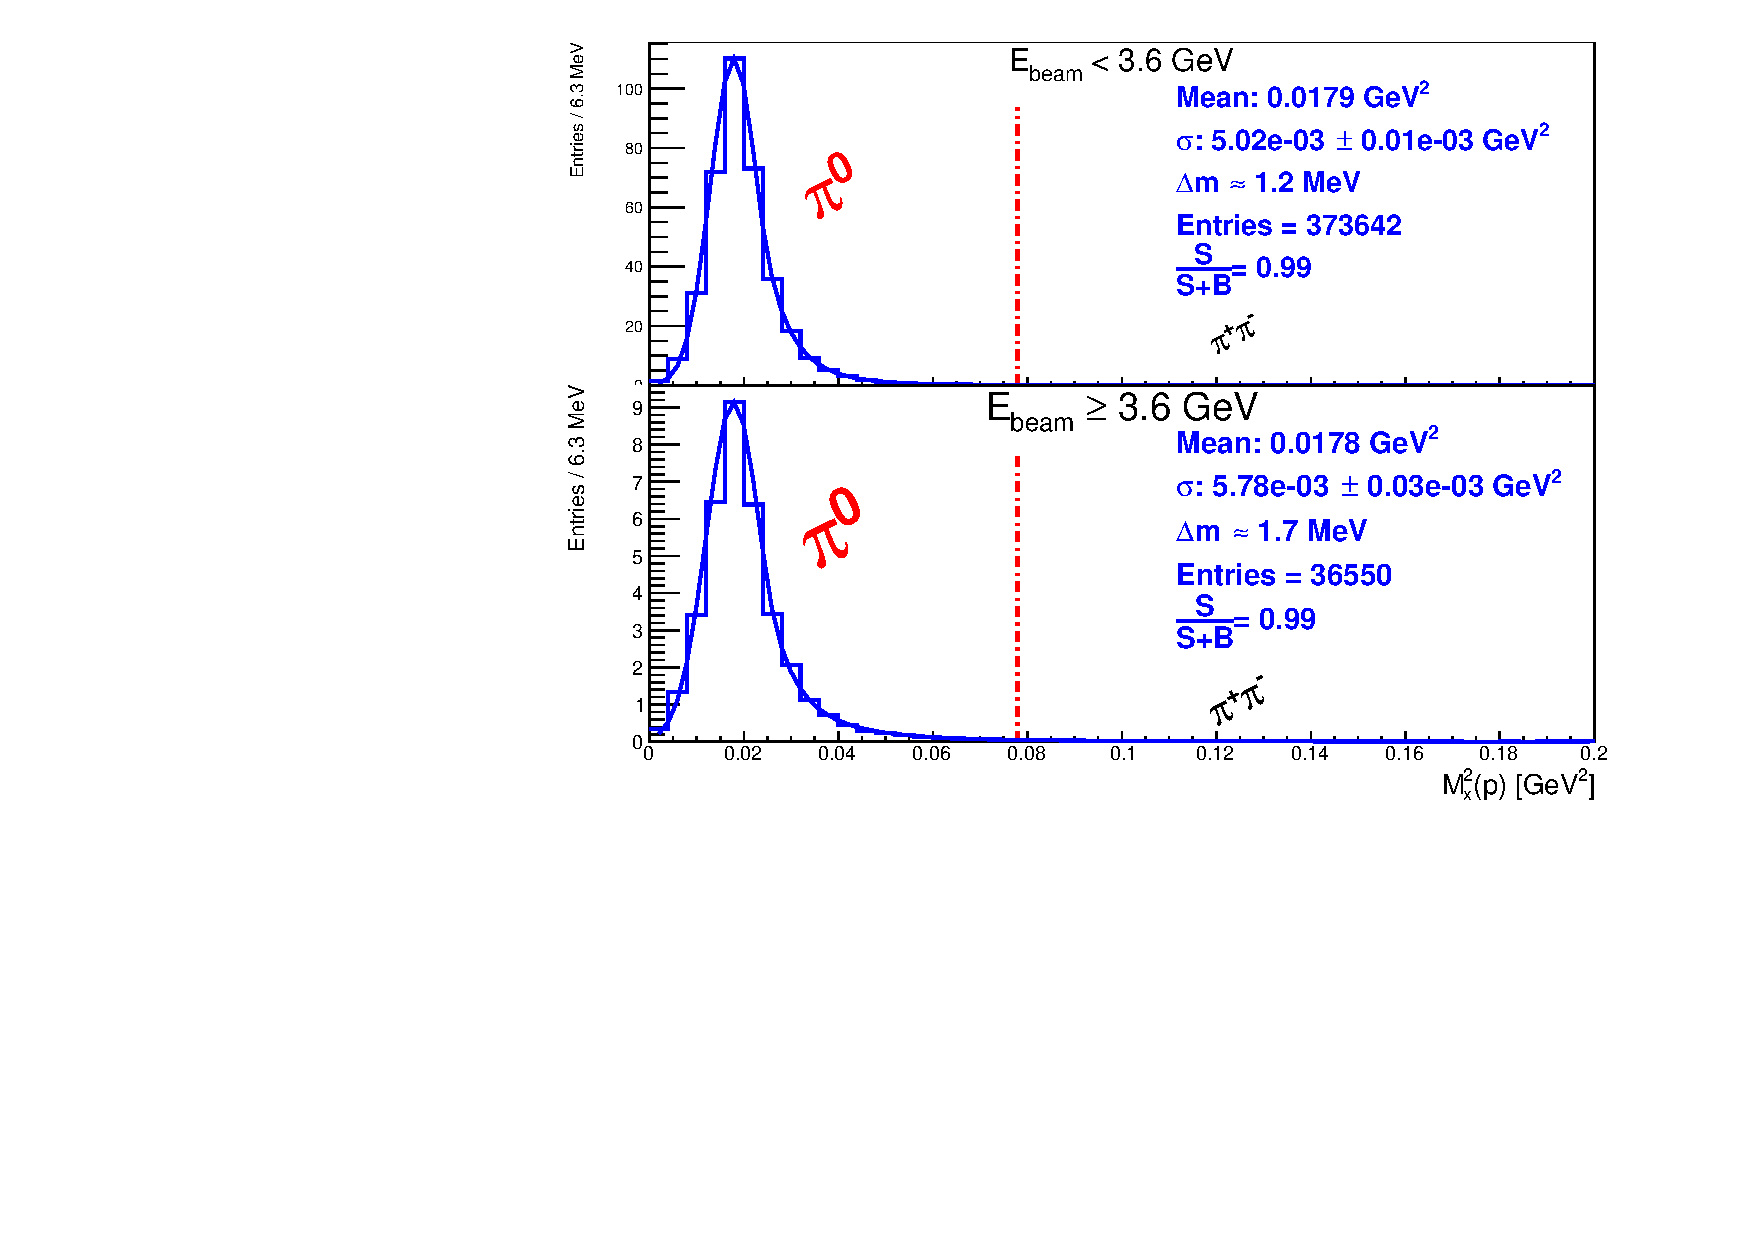
\includegraphics[width=\figwidth,height= 0.75 \hfigheight]{\figures/analysis/KineFitter/DATA/hdataLEP_MOR_pi0_FINAL_PLOTS.pdf}
\caption[Number of data events plotted vs. missing mass $M_x(\gamma p \to p X)$ for $\gamma p \to p e^+ e^- (\gamma)$ events after all cuts and corrections.]{\label{fig:kinfit.final.plot}Number of data events plotted vs. missing mass $M_x(\gamma p \to p X)$ for $\gamma p \to p e^+ e^- (\gamma)$ events after all cuts and corrections.}
\end{center}\end{figure}
\FloatBarrier
